\definecolor{cfwone}{HTML}{eef5fa}
\definecolor{cfwtwo}{HTML}{daeaf5}
\definecolor{cfwthree}{HTML}{b2d2e9}
\definecolor{cfwfour}{HTML}{8abbde}

\newcommand{\fwone}[1]{\colbox{cfwone}{#1}\xspace}
\newcommand{\fwtwo}[1]{\colbox{cfwtwo}{#1}\xspace}
\newcommand{\fwthree}[1]{\colbox{cfwthree}{#1}\xspace}
\newcommand{\fwfour}[1]{\colbox{cfwfour}{#1}\xspace}

\newcommand{\fexp}[2]{\texttt{[{\color{darkgray}{#1:#2}}]}\xspace}
\newcommand{\fexptag}[1]{\fexp{TAG}{#1}}
\newcommand{\fexpfrom}[1]{\fexp{FROM}{#1}}
\newcommand{\fexpto}[1]{\fexp{TO}{#1}}
\newcommand{\fexptemp}[1]{\fexp{TEMP}{#1}}


\section{Counterfactual Explanations}
\label{sec:app_explain}
%Both counterfactual explanations and semi-counterfactual explanations.
%As defined in \cite{}






\begin{figure}[t]
\centering
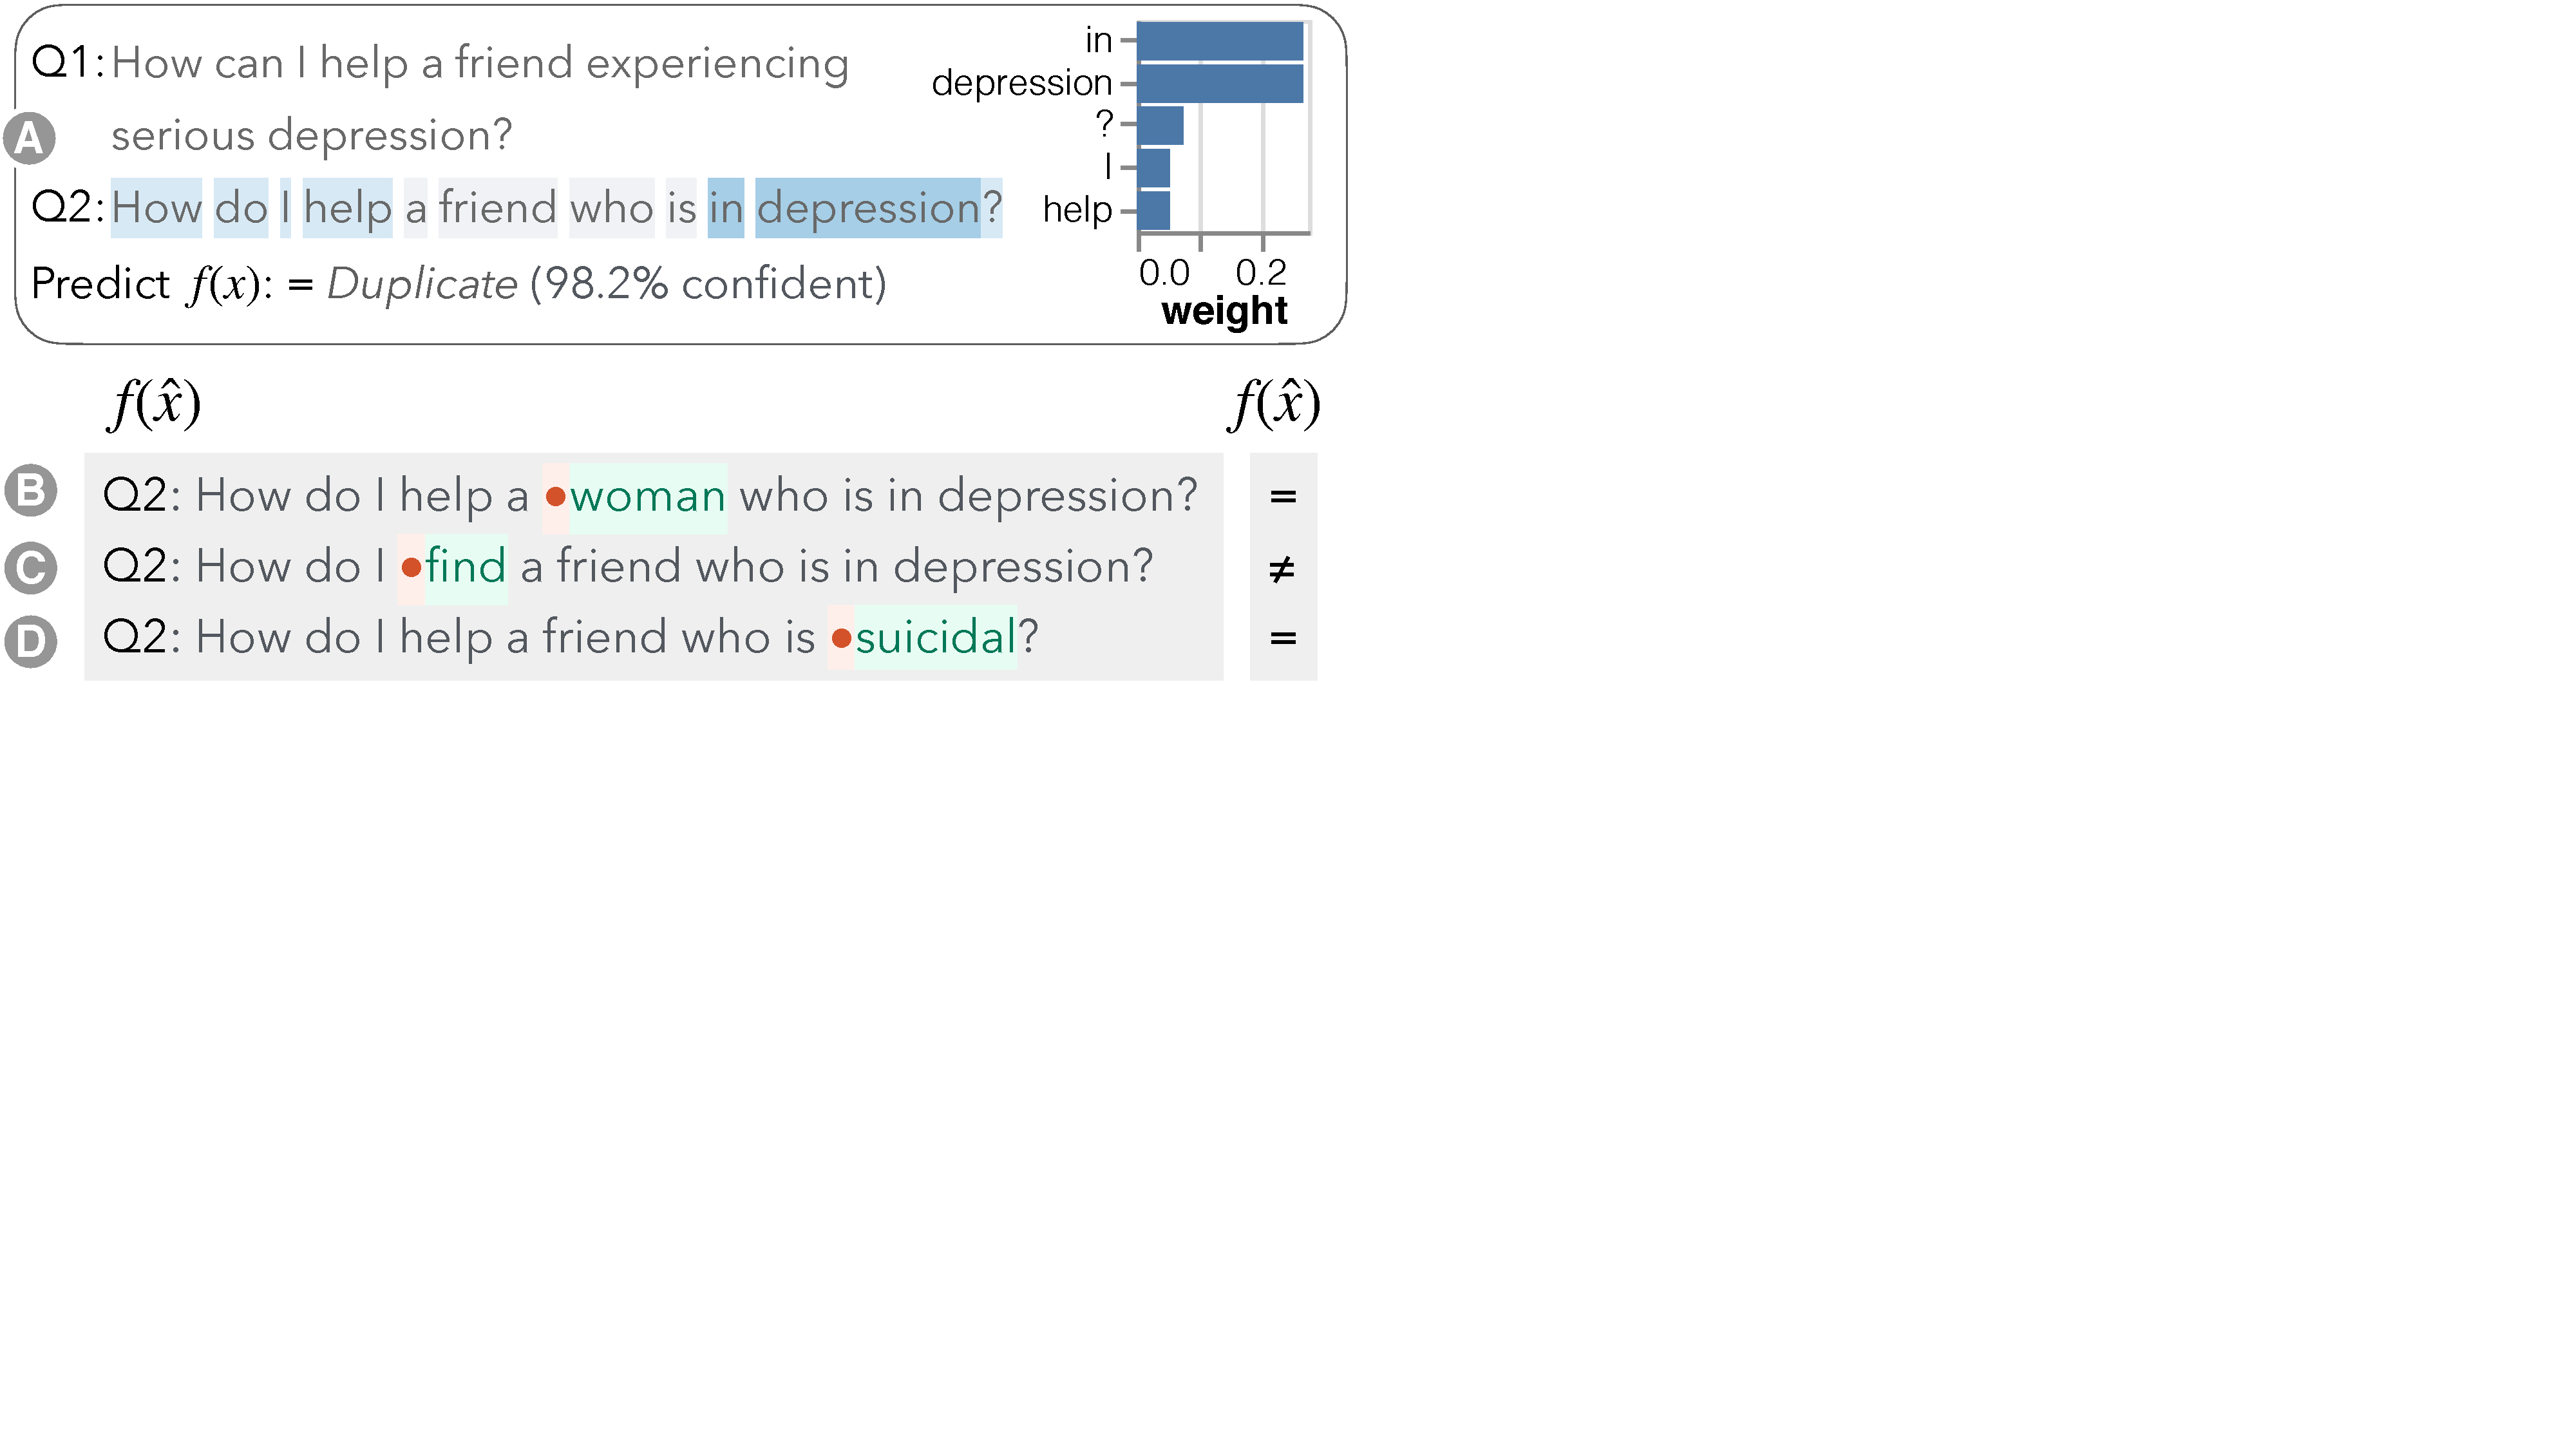
\includegraphics[trim={0 20cm 32cm 0cm},clip,width=1\columnwidth]{figures/explanation_v2}
\vspace{-15pt}
\caption{
Counterfactual explanations on a \qqp instance (A), which compensates the feature weights from SHAP visualized by the blue backgrounds and the bar chart.
Counterfactuals can 
(B) concretize the opaque weights using readable examples. so it is more noticeable that the model does not recognize ``reasons'';
(C) alert errors missed by SHAP, so users are not misled to believe that the model will respond correctly to changed person names.
\wts{highlight B in main text? And maybe a less political example?}
}
\vspace{-10pt}
\label{fig:explanation}
\end{figure}

%\wts{Finding bugs missed by the feature attribution, and concretizing the opaque weights using readable examples.}
\subsection{Selections for Different Explanations}

Compared to feature attribution methods, counterfactual explanations more intuitively answer users' implicit ``why P rather than Q'' questions~\cite{miller}.
If we are 


\paragraph{Local explanations: Abnormality.}
%Compared to feature attribution methods, counterfactual explanations more naturally answer users' 
The cognitive burden of complete explanations around one instance is too great.
As a result, \citet{miller} concluded that people usually \emph{select} a small subset of (counterfactual) explanations on contrastive cases (``foils'') that they find unexpected. 
As such, he further proposed that ``abnormality could be used to infer likely foils.''
Here, we operationalize the concept of abnormality based on \emph{the discrepancy between the expected and the actual changes in the prediction}, and use it as our selection method.

Given a prediction model $f$, we define the actual change in prediction as $d_f(\xp, x)$, and the expected prediction change as $\hat{d}_f(\xp, x)$.
The distance between the expectation and reality then becomes:
$$\Delta d_f(\xp, x) = |\hat{d}_f(\xp, x)-d_f(\xp, x)|$$
We select two abnormal, ``turning point'' counterfactuals, \ie unexpected large gap in prediction when the perturbation is considered minimal $\argmax_{\xp} \Delta d_f(\xp, x)$, or the unexpected small prediction changes $\argmin_{\xp} \Delta d_f(\xp, x)$.

Whereas $d_f(\xp, x)=|f_p(\xp)-f_p(x)|$ where $f_p(x)$ denotes the prediction probability of $f$ on $x$, $d_f(\xp, x)$ can take various forms. 
As a standalone explanation method, it can be the cosine distance in the \emph{Embedding space}.
The embedding can be either model-agnostic (\eg with~sentence transformers~\cite{reimers-2019-sentence-bert}), or the last layer of the hidden state of the finetuned predictor.

On the other hand, as a \emph{compensation} to existing feature attribution methods, $\hat{d}_f$ can be the importance (weights) of the perturbed tokens in $x$, estimated by feature attribution methods.
As mentioned in \S\ref{sec:relate}, methods like SHAP or LIME only estimate feature weights by \emph{masking} the words, and therefore do not reflect how model would react in non-deletion counterfactuals (replacing words or inserting negations).
However, the nuance is usually lost on an average SHAP/LIME user.
Therefore, abnormalities selected in this way can compensate or criticize the missed information, and better calibrate users' trust on the predictor. 
Detailed distance functions are in \tofix{\S\ref{X}}.
\wts{Add appendix}



\paragraph{Interactive explanations: Targeted Foils}
%\paragraph{Interactive explanation.}
Automatically selected explanations point to general abnormality, but users should be able to specify a foil to implicitly point towards the part of the model \emph{they} do not understand~\cite{miller}.
%Furthermore, the method should allow explanations as a dialog. 
The targeted generation seamlessly support such interactive explanation (ideally in a visual interface), and multi-step drill downs.
For example, to inspect model responses to entities, an analyst can blank ``Hillary'' in Figure~\ref{fig:explanation} Q2 to get additional human names.
Or, they may keep the change ``Trump'' in Figure~\ref{fig:explanation}B, and further blank ``dislike'' to see how the model reacts to \add{hate} or \add{love} \add{Trump}.


\paragraph{Global Explanations: Recurring Edits}
\label{subsec:global_exp}
%\paragraph{Global explanations: impacts of same changes.}
Besides abnormality around an individual data point, \emph{global} ones provides more systematic observations, and therefore brings more generalizable model understandings --- yet another important aspect of model explanations~\cite{miller}.
We find \emph{abnormal groups} of counterfactual through two steps: 

First, we featurize counterfactuals to create groups of similar changes. 
The featurization uses, like the \tagstr between $\xp$ and $x$, the edited spans, etc.
%(1) its \tagstr (\fexptag{negation} for the example in Figure~\ref{fig:blank}), 
%(2) its remove phrases \fexpfrom{kids}, 
%(3) its added phrases \fexpto{not}, \fexpto{children}, and 
%(4) the combined template \fexptemp{\swap{kids}{children}}.
Then, we rank the groups $G = \{ \xp_1, \xp_2, ...\}$ using the entropy of the prediction changes $(f(x) \rightarrow f(\xp))$ for all counterfactuals in a group.
Intuitively, larger entropy indicates that the perturbation has unstable impact on the prediction.

For example, when evaluating the \nli RoBERTa model (the same as in \S\ref{subsec:contrast_set}), one abnormal global perturbation is \swap{two}{three} in the hypothesis.
Out of the 253 counterfactuals whose original prediction $f(x)=$ \emph{entailment}, $138$ flipped to \emph{contradiction}, $22$ to \emph{neutral}, yet $93$ remained \emph{entailment}, resulting in entropy $I=0.91$.
We observe that most cases flipped to \emph{contradiction} have the explicit word ``two'' in the premise, whereas the prediction-intact ones suggest that the model cannot process actual counting.

\ebox{
\textbf{P}: Two women having drinks at the bar.\\
\textbf{H}: \swap{Two}{Three} women are at a bar.\\
\textbf{$\mathbf{f(x)\rightarrow f(\xp)}$}: \swap{entailment}{contradiction}\\
--\\
\textbf{P}: A boy and a girl gaze in a clothing store window.\\
\textbf{H}: \swap{Two}{Three} kids are looking in a store window.\\
\textbf{$\mathbf{f(x)\rightarrow f(\xp)}$}: \swap{entailment}{entailment}
}


\subsection{Local Exp.: Complement SHAP?}
Here, conduct a user study to verify whether our local counterfactual explanations can compensate SHAP in helping people interpret the model, \ie if the selected counterfactual spot points that people would mis-interpret after viewing SHAP.
The setup nicely combines the overview provided by SHAP/LIME, and the decision boundaries omitted by the feature attribution. 
We defer more sophisticated designs and evaluations for interactive and global explanation to future work.

We form the study as a counterfactual simulation on the model's behavior~\cite{hase2020evaluating}, where participants are asked to predict model's behavior on the given variations of a reference example.
Intuitively, the more counterfactuals they simulate incorrectly, the more information they grasp \emph{if we show the counterfactuals to them}.

\paragraph{Procedure.}
We recruited \tofix{N} graduate students who have taken at least one NLP course, and have experience using model explanations before, and asked them to simulate the behavior of a \qqp model for 20 rounds (the same as in \S\ref{subsec:contrast_set}).
In each round, the participants were given a reference example, with the model's prediction on it, its confidence score, as well as the feature attributions estimated by SHAP (Figure~\ref{fig:explanation}A).
To help them better understand the model around the reference example, the participants were allowed to ``query the model'' for up to 10 times, by making small changes to one question, and see the resulting model predictions.
It was equivalent to unlimited model access --- participants submitted \tofix{$6.9\pm3.0$} queries.
More interactions with the model usually results in better mental models about the predictor~\cite{miller}, and we are interested in whether our selected ones \emph{still add information} on top of such mental models.
Participants were then asked to simulate the model's prediction on six counterfactuals (Displayed similar to Figure~\ref{fig:explanation}B), two from each condition.
We concluded the study with open-ended questions on their model query and simulation strategies.

\newcommand{\cshap}{\emph{SHAP-c}\xspace}
\newcommand{\crandom}{\emph{Random}\xspace}
\newcommand{\chuman}{\emph{Human}\xspace}

\paragraph{Conditions.} 
We compare three types of selected counterfactuals:
(1) \cshap, the machine-generated counterfactuals selected to compensate SHAP; 
(2) \crandom, the randomly selected machine-generated counterfactuals; 
(3) \chuman, 
the human generated counterfactuals that they deemed abnormal.
We allowed three graduate students to play with the model for up to 10 times, and asked them to submit one final counterfactual with a surprising model prediction.
We then randomly selected two of their submissions per reference example.
As a within-subject study, we compared the error rate of human simulations across the three conditions.


\begin{figure}[t]
\centering
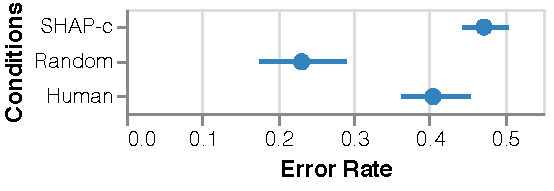
\includegraphics[width=1\columnwidth]{figures/exp_err_rate}
\vspace{-15pt}
\caption{
Error rates on counterfactuals in different conditions. The higher the error rate, the more information missed by the participants (\ie and therefore can better complement model interactions and SHAP.)
}
\vspace{-10pt}
\label{fig:err_rate}
\end{figure}

\paragraph{Results.}
As in Figure~\ref{fig:err_rate}, participants performed well on \crandom (error rate $e=23\%\pm7\%$) but poorly on \cshap ($47\%\pm 4\%$).
While SHAP and model interactions indeed helped experts simulate model behaviors on some counterfactuals, \cshap counterfactuals were beyond their mental models, and \emph{would still add value if they were presented as part of the explanation.}

Participants also missed many \chuman counterfactuals ($40\%\pm 5\%$), though it was expected --- these cases were surprising even to their human creators.
Their performance on \chuman were slightly better than on \cshap, indicating that \emph{SHAP-c were at least as surprising as the Human selected abnormal cases.}

More interestingly, their poor performances on the two conditions were for different reasons: 
%\ie \emph{Missing inspections v.s. Missing bugs within an inspected spots.}
When participant mis-predict a \cshap counterfactual $\xp$, \tofix{80\%} of the time, they covered the related pattern in their model interaction (\ie $>75\%$ of the changed tokens in $\xp$ were also changed in at least one of their queries), and the number dropped to \tofix{$62\%$} in \chuman.
This indicates that, compared to \chuman where participants missed the inspection spots of another human creator (and therefore had to ``guess using intuitions''), they were \emph{misled} by their inspections in \cshap --- ``I give the same prediction as the similar example I tried'', as one subject articulated.
For example, when the model predicted \emph{Duplicate} on their query \exinline{How do you overcome \add{your} emotional attachment?}, it was hard for them to imagine model predicting \emph{Duplicate} on \exinline{How do you overcome \add{this} emotional attachment?} 
In other words, \emph{SHAP-c found more bugs within spots where humans considered inspected, which is a different bug space compared to the human selected abnormality.}

Moreover, in their freeform responses, \tofix{3 out of 7} participants mentioned they prioritized perturbing words with high feature weights, which further indicated the importance of selecting \emph{unexpected prediction change} for them.


